\quad The origin of our project lies in a FEDs note dated October 2022\cite{savingsfed}. Their work aimed at estimating the \textit{‘excess savings’} - savings accrued during the pandemic as spending opportunities in either goods or services were severely curtailed – accumulated through 2020 and the first semester of 2021 by American households compared to what would have happened if income and spending components had growth at pre-pandemic trends, in short, compared to a no Covid-19 crisis counterfactual. The computation of excess savings is done following a detailed accounting approach. We build on their work and extend their methodology to European households, precisely we estimate excess savings for the European Big 4 (France, Germany, Spain and Italy), the UK and also the US for our purposes. Regarding the latter, comparing with the Fed’s work allows us to see that we are in line when it comes to variable choices and methodology.\par
The subject of excess savings has received a lot of attention for multiple reasons. It is a high-profile news topic as it concerns any household but more importantly, the outlook for economic growth, inflation, household welfare and consumption heavily depends on the amount of savings to consider and especially who holds it. Thus, after displaying the methodology and different variables used for the 6 countries of our study, we assess the recent drivers that led to the soaring of the personal saving rate and estimate the different contributions. In addition to the raw aggregate excess saving number for the whole economy, we were also interested in estimating a distribution of the latter across the population and assessing in what asset form these savings were held.

\subsection{Methodology and Variable choices}
\quad We aim at estimating the aggregate amount of excess savings. As a reminder, we worked on this project in early Q1 2023 and as we still lacked data for Q4 2022 results are up until Q3. The ‘Flow of savings’ can be written as: 
\begin{align*}
    \resizebox{.9\hsize}{!}{\textit{\mbox{Flow of savings} = \mbox{Disposable Personal Income} - \mbox{Personal Consumption Expenditures} - \mbox{other outlays}}}
\end{align*}   
\vspace{-0.05cm}
\quad We compute the disposable personal income (DPI) -the income available to households- as the compensation of employees (which takes into account not only wages and salaries in cash or in kind paid to the employee but also the employer’s imputed social contributions) \textbf{plus} received income from social transfers in kind and property \textbf{less} taxes on income, paid property income and other current transfers paid. 
We get data from multiple different sources: Eurostat and national sources for European countries; the Office for National Statistics for the UK; and the Federal Reserve database for the US. These different sources led us to different ways to compute the Disposable Personal Income. 
The details for every country can be found in the annexe (Figure \ref*{figure:DPI_table}). We checked with every regional economist if we had chosen the correct variables or had missed anything.
To calculate the quarterly flows of excess savings we look at the difference between ‘excess’ disposable income and the ‘shortfall’ of consumption both relative to their pre-pandemic (2015-19) log-linear trend from Q1 2020 onwards (see Figure \ref{figure:fr_compensation} for an illustrative example with the compensation of employees in France). 
Similarly to the Fed's original paper, every component of the personal income is measured in Nominal national currency, this assumes that both nominal and real values move along their pre-pandemic trends. 
Thus, for every DPI component and personal consumption (PCE), we compute the difference (deviation) between the observed value and the counterfactual pre-pandemic trend (Figure \ref{figure:fr_compensation}). 

\subsection{Total stock of excess savings estimation}

For every country of the study, the left panels of Figure \ref{figure:Flows1} \& \ref{figure:Flows2} show the flows of excess savings, and the different components' contribution, over time and the right panels show the accrued stock.

\begin{figure}[H]
    \centering
    \caption{\textit{Flows of Excess Savings’ breakdown \& Cumulated Stock. \\ In order: France, Germany, Spain, Italy. Y-axis is in Billion Euros (EUR).}}
    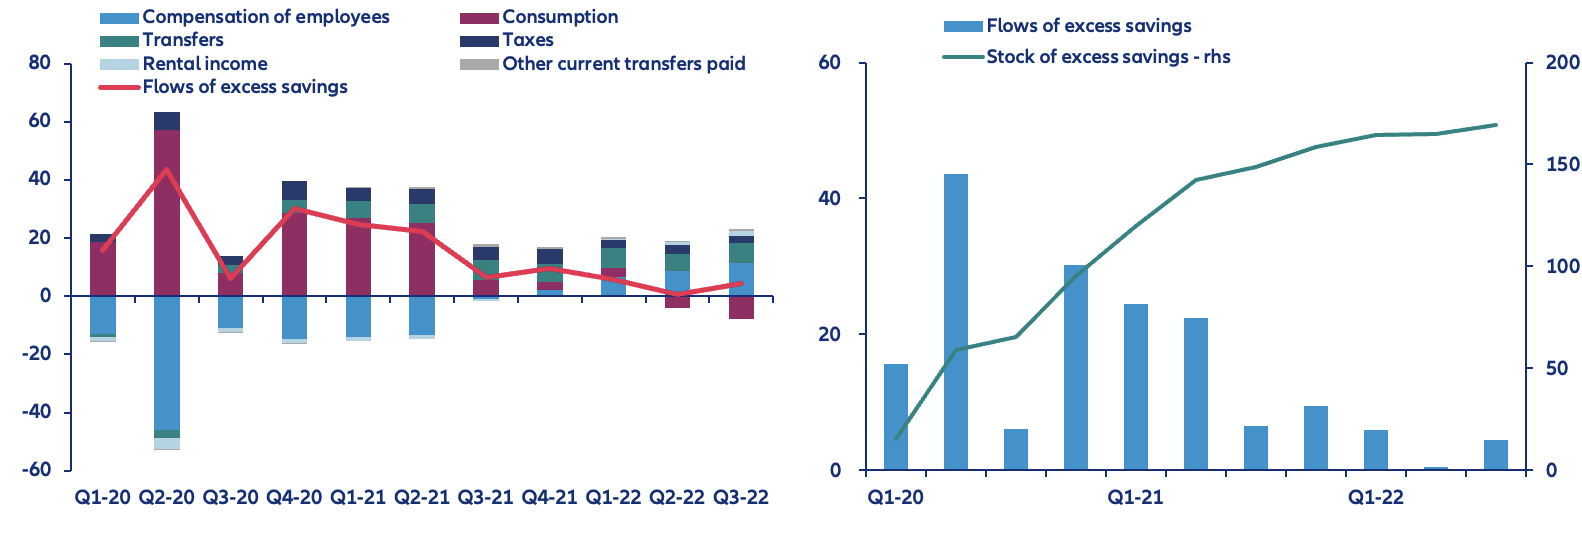
\includegraphics[width=.9\textwidth]{Core/1.Savings/img/xFrance.png}
    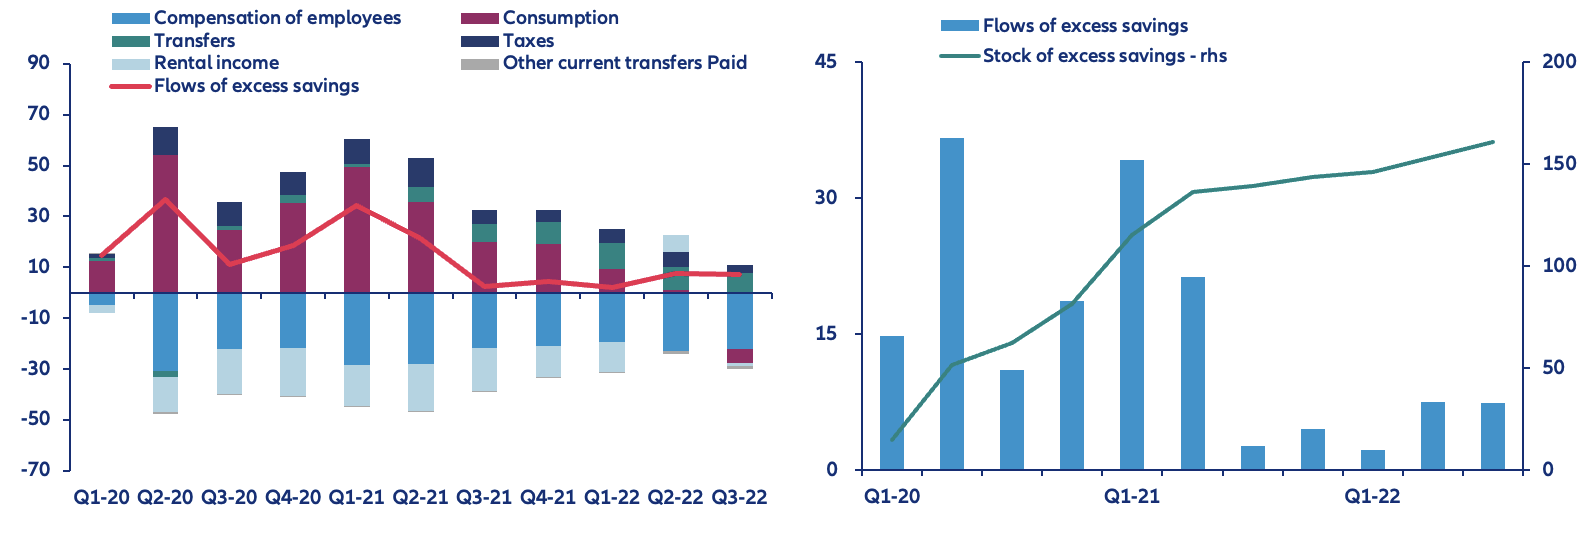
\includegraphics[width=.9\textwidth]{Core/1.Savings/img/xGermany.png}
    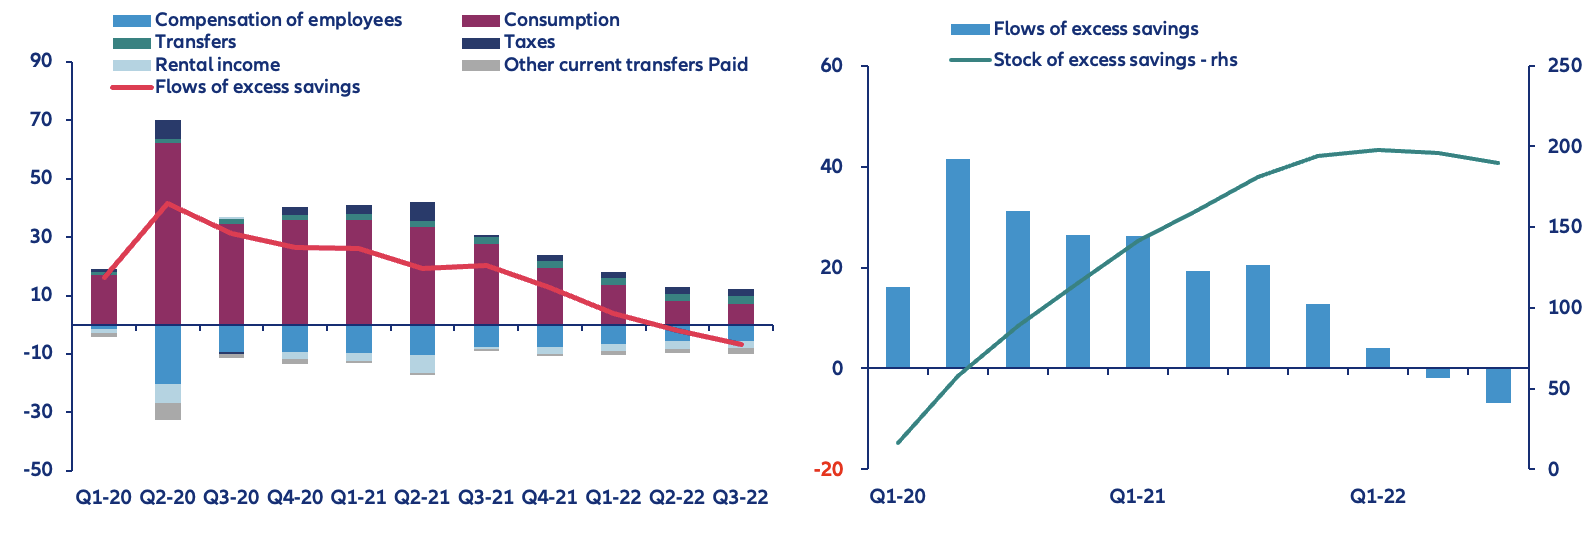
\includegraphics[width=.9\textwidth]{Core/1.Savings/img/xSpain.png}
    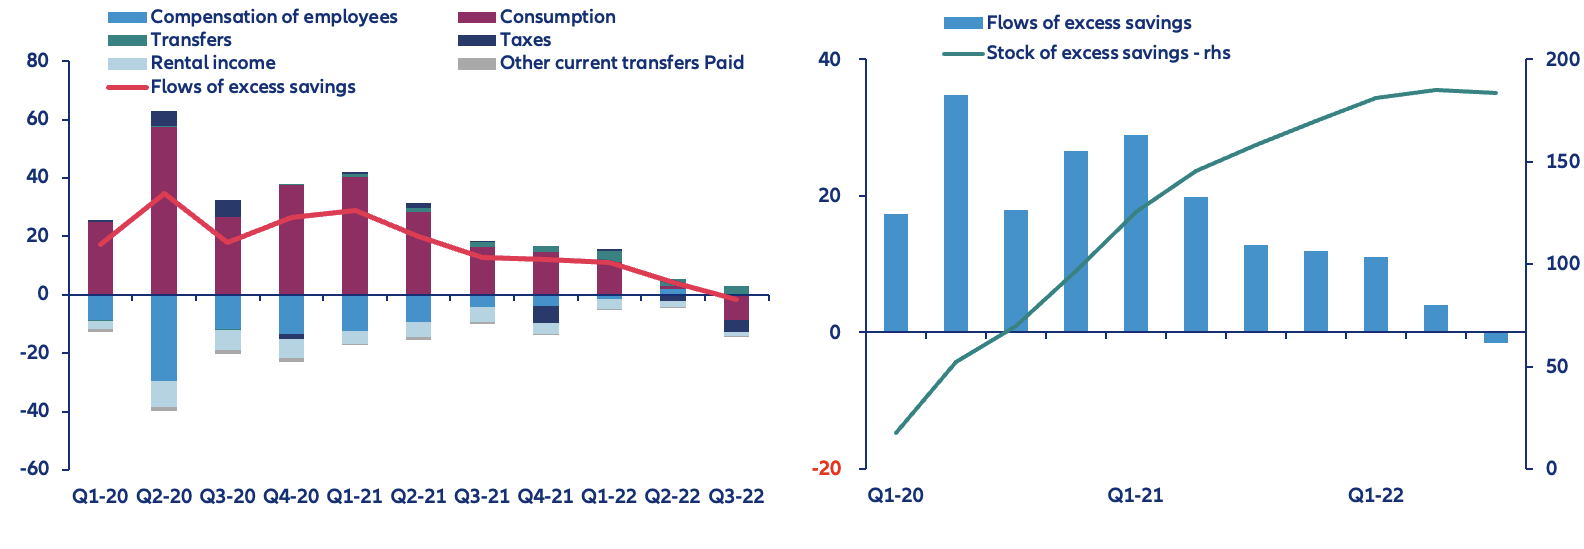
\includegraphics[width=.9\textwidth]{Core/1.Savings/img/xItaly.png}
    \label{figure:Flows1}
\end{figure}

\begin{figure}[H]
    \centering
    \caption{\textit{Flows of Excess Savings’ breakdown \& Cumulated Stock. \\ In order: the UK, the US. Y-axis is in Billion Local Currency Units (LCU).}}
    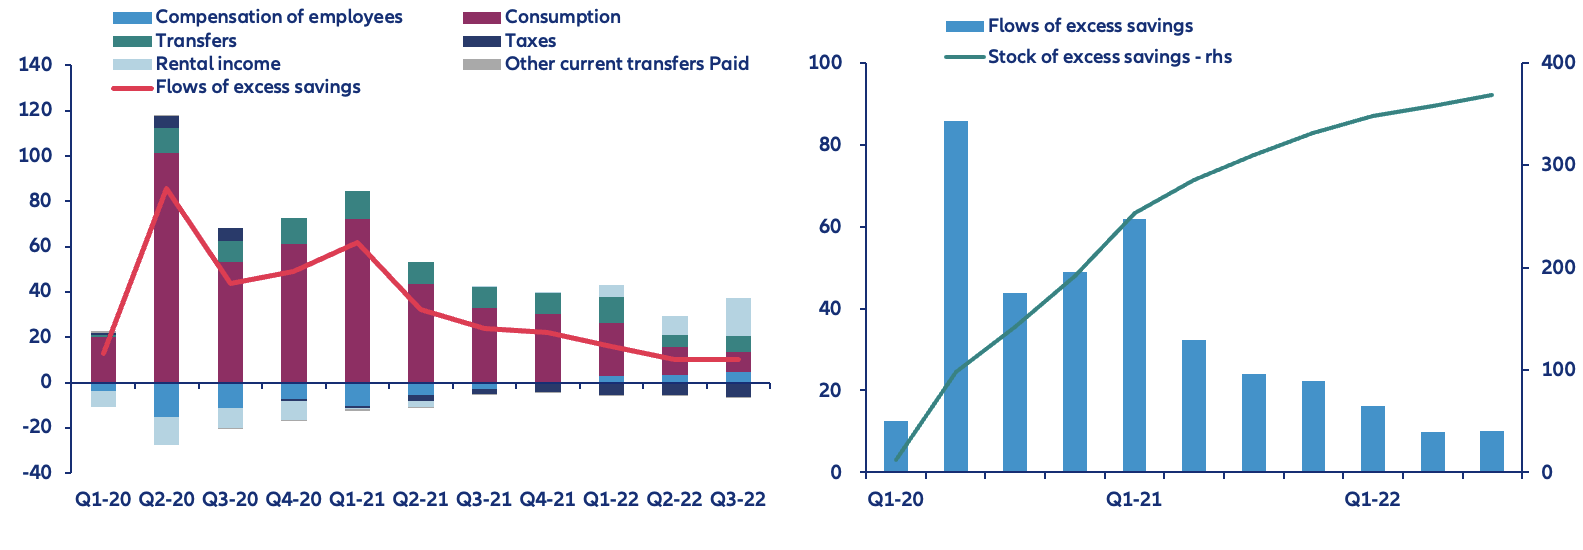
\includegraphics[width=.9\textwidth]{Core/1.Savings/img/xUK.png}
    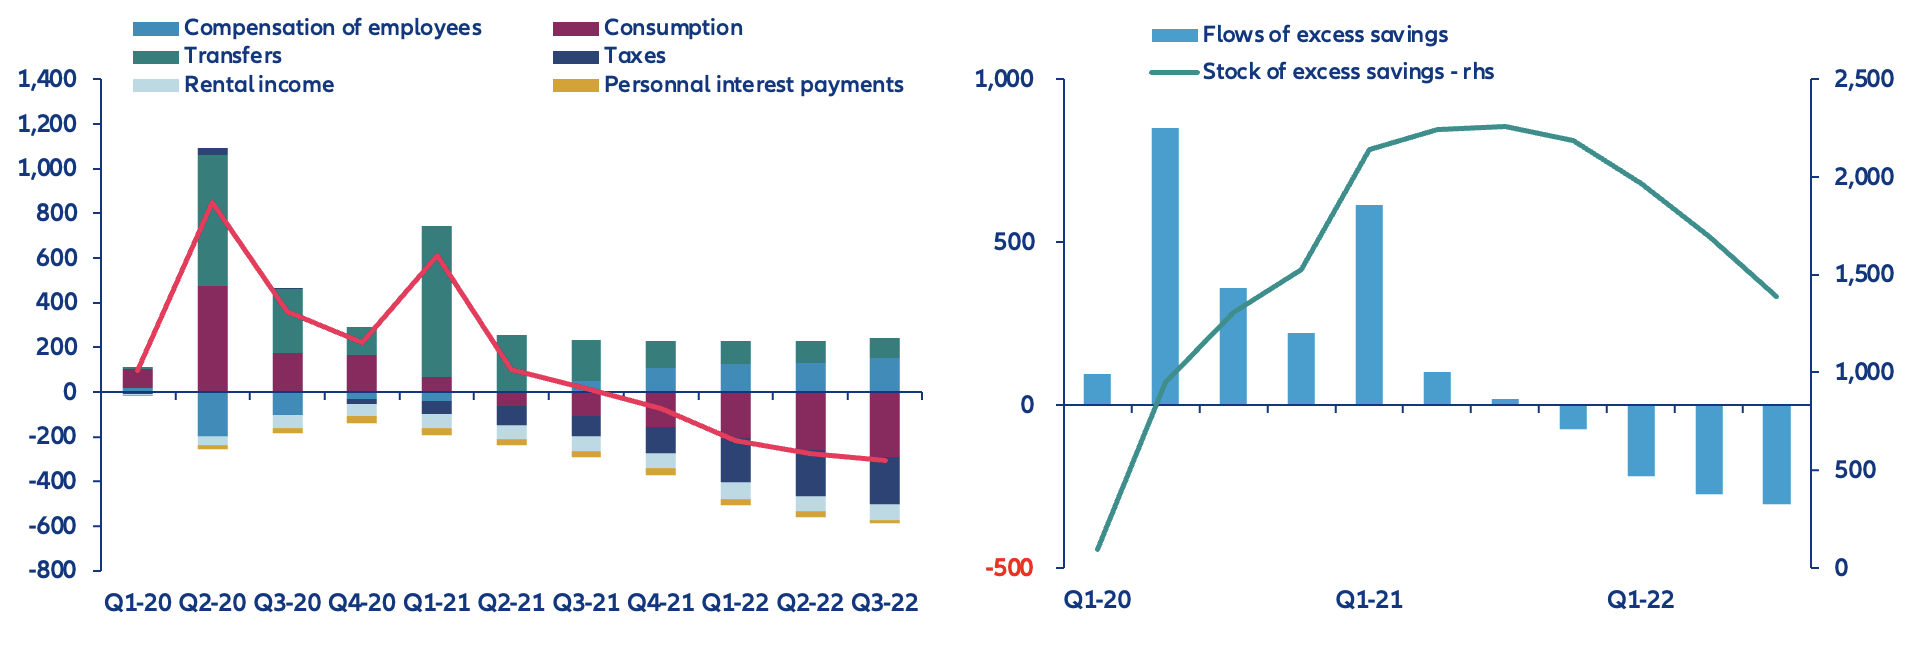
\includegraphics[width=.92\textwidth]{Core/1.Savings/img/xUS2.png}
    \label{figure:Flows2}
\end{figure}

The result of this exercise clearly shows that households have accumulated large savings throughout the pandemic in 2020 as incentives to consume were deeply curbed, especially during the different lockdowns. 
In addition to reduced expenditures in personal consumption, households’ disposable income has been boosted by fiscal transfers, particularly in the US. 
Disruptions in the different labour markets led to below pre-pandemic trend compensation of employees. As the markets normalised and tightened, increasing pressures on nominal wages drove up nominal compensation. 
Only the compensation of employees in Germany seems to remain below the pre-pandemic trend in level, while it returned to the trend in growth terms (see Figure \ref{figure:ger_compensation}). 
According to our computations, the stock of excess savings made up close to 25\% of annual consumption in the UK and Spain towards the end of 2022, i.e. GBP 370bn in the UK and EUR 190bn in Spain. 
Excess savings are lower as a share of consumption in France and Italy, but still large, at EUR 175bn and 185bn, respectively. 
In the US and Germany, however, the stock of excess savings ended 2022 at around 8\% of annual consumption, ie USD 1390bn in the US and EUR 160bn in Germany.

Excess savings shot up in 2020 and early 2021, despite lower aggregate compensation of employees compared to the pre-pandemic trend, mainly through heavily reduced personal expenditures for European countries (the UK included) and strong state support in the US, as huge fiscal transfers bolstered households’ balance sheet. 
According to our computations, between Q1 2020 and Q4 2021 the stock of households reduced spendings amounts to EUR 173Bn in France, 251Bn in Germany, 246Bn in Italy, 267Bn in Spain and GBP 414Bn. 
In the US, it peaked at US 971Bn in late Q1 2021 before starting depleting onwards, down to US 647Bn in Q4 of that year.
We estimate that in the span of two years (2020-2021), the state fiscal support buoyed US household income up to 2 trillion dollars (for reference President Biden's infrastructure plan unveiled in early 2021 was about the same amount). 
As of Q3 2022, quarterly transfer receipts remain above what the pre-pandemic trend would have suggested. 
However, since Q3 2021, excess savings in the US have been rapidly depleting (negative flows), while other countries at most showed lowering flows but still positive around that time. 
It appears that, amid consumption recovery, the strength of households’ consumption grew above the pre-pandemic trend (negative flows of consumption in the breakdown of excess savings Figure \ref{figure:Flows2} chart 2) and they have been digging into their pandemic excess savings to, on the one hand, fund their expenditures after the lockdown periods, but on the other hand also face rising inflation, which started picking from 1.2\% in Q4 2020 to almost 7\% in Q4 2021. 
Still, households continued purchasing more \textit{volumes} of goods and services despite elevated inflation. 
This explains the fast depletion of excess savings and with the savings rate settling around 3\% in Q3 and Q4 2022, much below the pre-pandemic trend, the stock of excess savings could be fully depleted by the end of the year. 
With the fear of recession for the US, households disposable income could be under further stress despite falling inflation and steep up the dig up of remaining excess savings.

Conversely, it appears that consumption recovery in Europe remained subdued with decreasing but positive and still large positive contribution of consumption throughout 2021 in the breakdown Figure \ref{figure:Flows1}.
As of Q3 2022 personal consumption expenditures still remain below the pre-pandemic trend in Spain and the UK, which explains why households in these countries have accumulated a large stock of excess savings. 
In other countries of the region consumption growth only returned to the levels suggested by the pre-pandemic trend around Q2 2022, long past the lockdown periods. 
Italian and Spanish households digging into their savings, despite what we have said regarding consumption, probably also reflects quickly rising inflation rates and increasing pressures on households’ finances. 
It is worth noting the taxes reduction bolstered households’ savings in European countries in both 2020 and 2021, while in the US increasing taxation from early 2021 onwards has been strengthening the dig up of savings to fund living expenses and increasing consumption.

With the aggregate figures estimated we assumed the country-specific excess savings distribution followed the total assets distribution across households. 
Through this we were able to give, for each quintile, an amount per household left as of Q3 2022 (see Figure \ref{figure:Savings}). 
Unexpectedly, it is very unevenly distributed, and we estimate the bulk of excess savings is held by the 20\% of households with higher income. 
On average, the top 20\% holds 65\% of excess savings vs. around 5\% for the bottom 40\% (and below 1\% for the bottom 20\% alone). 
The average high-income household has, on average, excess savings ranging from EUR 13,650 in Germany to GBP 41,600 in the UK. 
At the opposite end of the spectrum, the bottom 20\% of households have essentially no more excess savings left, except in the US where the average household has around USD 1,800 remaining. 

\begin{figure}[H]
    \centering
    \caption{\textit{Amount per household of excess savings remaining as of Q3 2023 (left panel, LCU) \& Total stock by quintile (right panel, LCU Bn)}}
    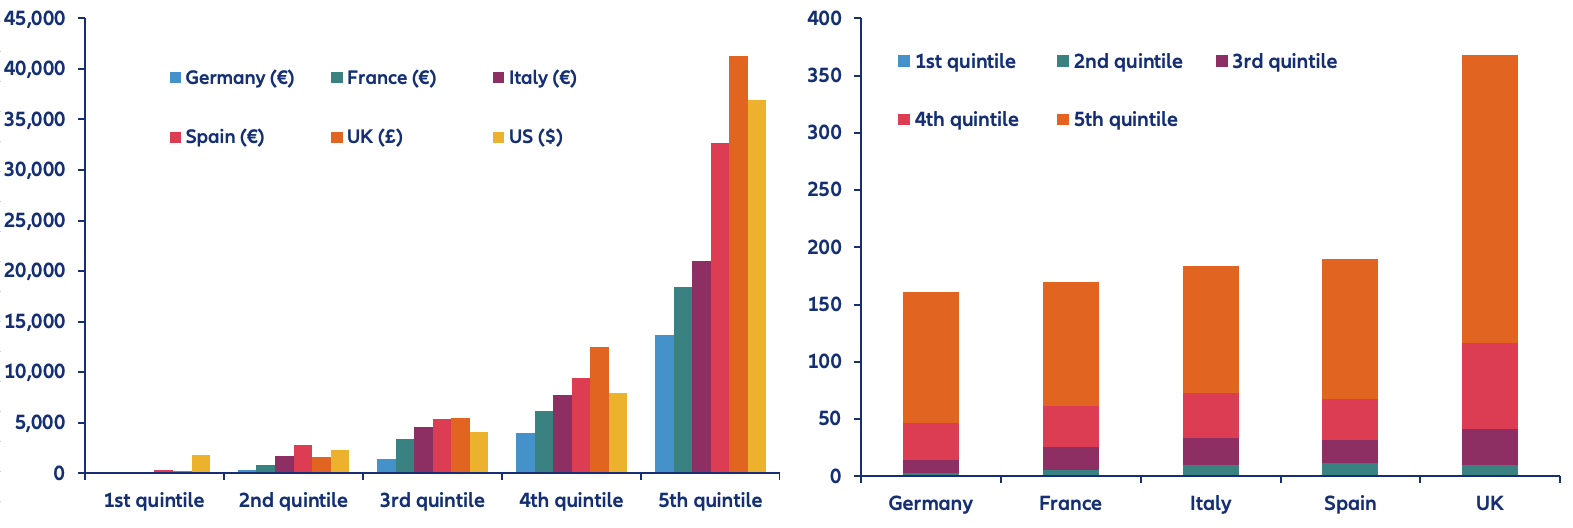
\includegraphics[width=1\textwidth]{Core/1.Savings/img/xSavings.png}
    \label{figure:Savings}
\end{figure}

\subsection{Excess savings' allocation towards asset classes}

\quad After estimating the aggregate stock of excess savings, and then an amount per household, we also attempted to work on a breakdown of the said stock per country across asset classes. 
In essence, we were interested in figuring out in what form these savings were held or if they were used towards paying off debt. To do so we had to come up with a methodology and formulate hypotheses. 
In hindsight, it may give some interesting elements to work with but it would need further work to be that effective. 
We used the household balance sheet from Eurostat for European countries, the Flow of Funds Financial Accounts from the National Office of Statistics for the UK and the households balance sheet from the Federal Reserve for the US. 
Assets held by households are mainly composed of Currency \& deposits; Equity \& IF shares; Insurance, pension \& stand guar; other account receivable;	debt securities and Gross fixed capital Formation. We assume households’ liabilities are only made of loans (accounts for 93.5\% of total households' financial liabilities in 2021 according to Eurostat). 
Below are the following rules we use to calculate the investments made by households. We agree they are quite harsh (probably erratic to some extent) and would need further discussion, but we had already figured out most of what we were looking for and just went on for some exploratory work that I still wished to include here as it was part of my learning.

- Assets: every quarter we only account for positive flows; meaning we assume that for any given variable if the quarterly flow is negative households did not allocate part of their excess savings towards that asset class (rather they cashed out).

- Loans: we only account for negative flows here; if loan flows are positive for a given quarter, then on average households contracted more debt than they paid back and we assume no share of excess savings were allocated to the reimbursement of debt. 
And conversely, if the flow is negative we assume on average households decided to invest towards the reimbursement of their debt: we take this flow into account. The investment made by households towards paying back their debt thus equals minus the negative flow. 

Thus, for any given quarter we assume that households' total investment is made of the assets positive flows and the liabilities negative flows: we are then able to derive a share of the total investment (\%) for each class. 
We assume that the allocation of excess savings in asset classes follows the same distribution as investment in these very own classes. 
We get households' excess savings distribution across asset classes at a given quarter by multiplying the flow of saving for that very own quarter by the corresponding previously computed share. 
We derive the savings stock breakdown by adding up the quarterly flows. According to our estimations, the most of excess savings (for European countries) is held in non-liquid forms, such as residential investment and equity: for instance, in Spain, currency and deposits account for 30\% of total excess savings, i.e. around EUR 60bn out EUR 195 bn (see Figure \ref{figure:SpainAL}). 

\begin{figure}[H]
    \centering
    \caption{\textit{Estimated breakdown of Spanish stock of excess savings (EUR bn) into asset classes}}
    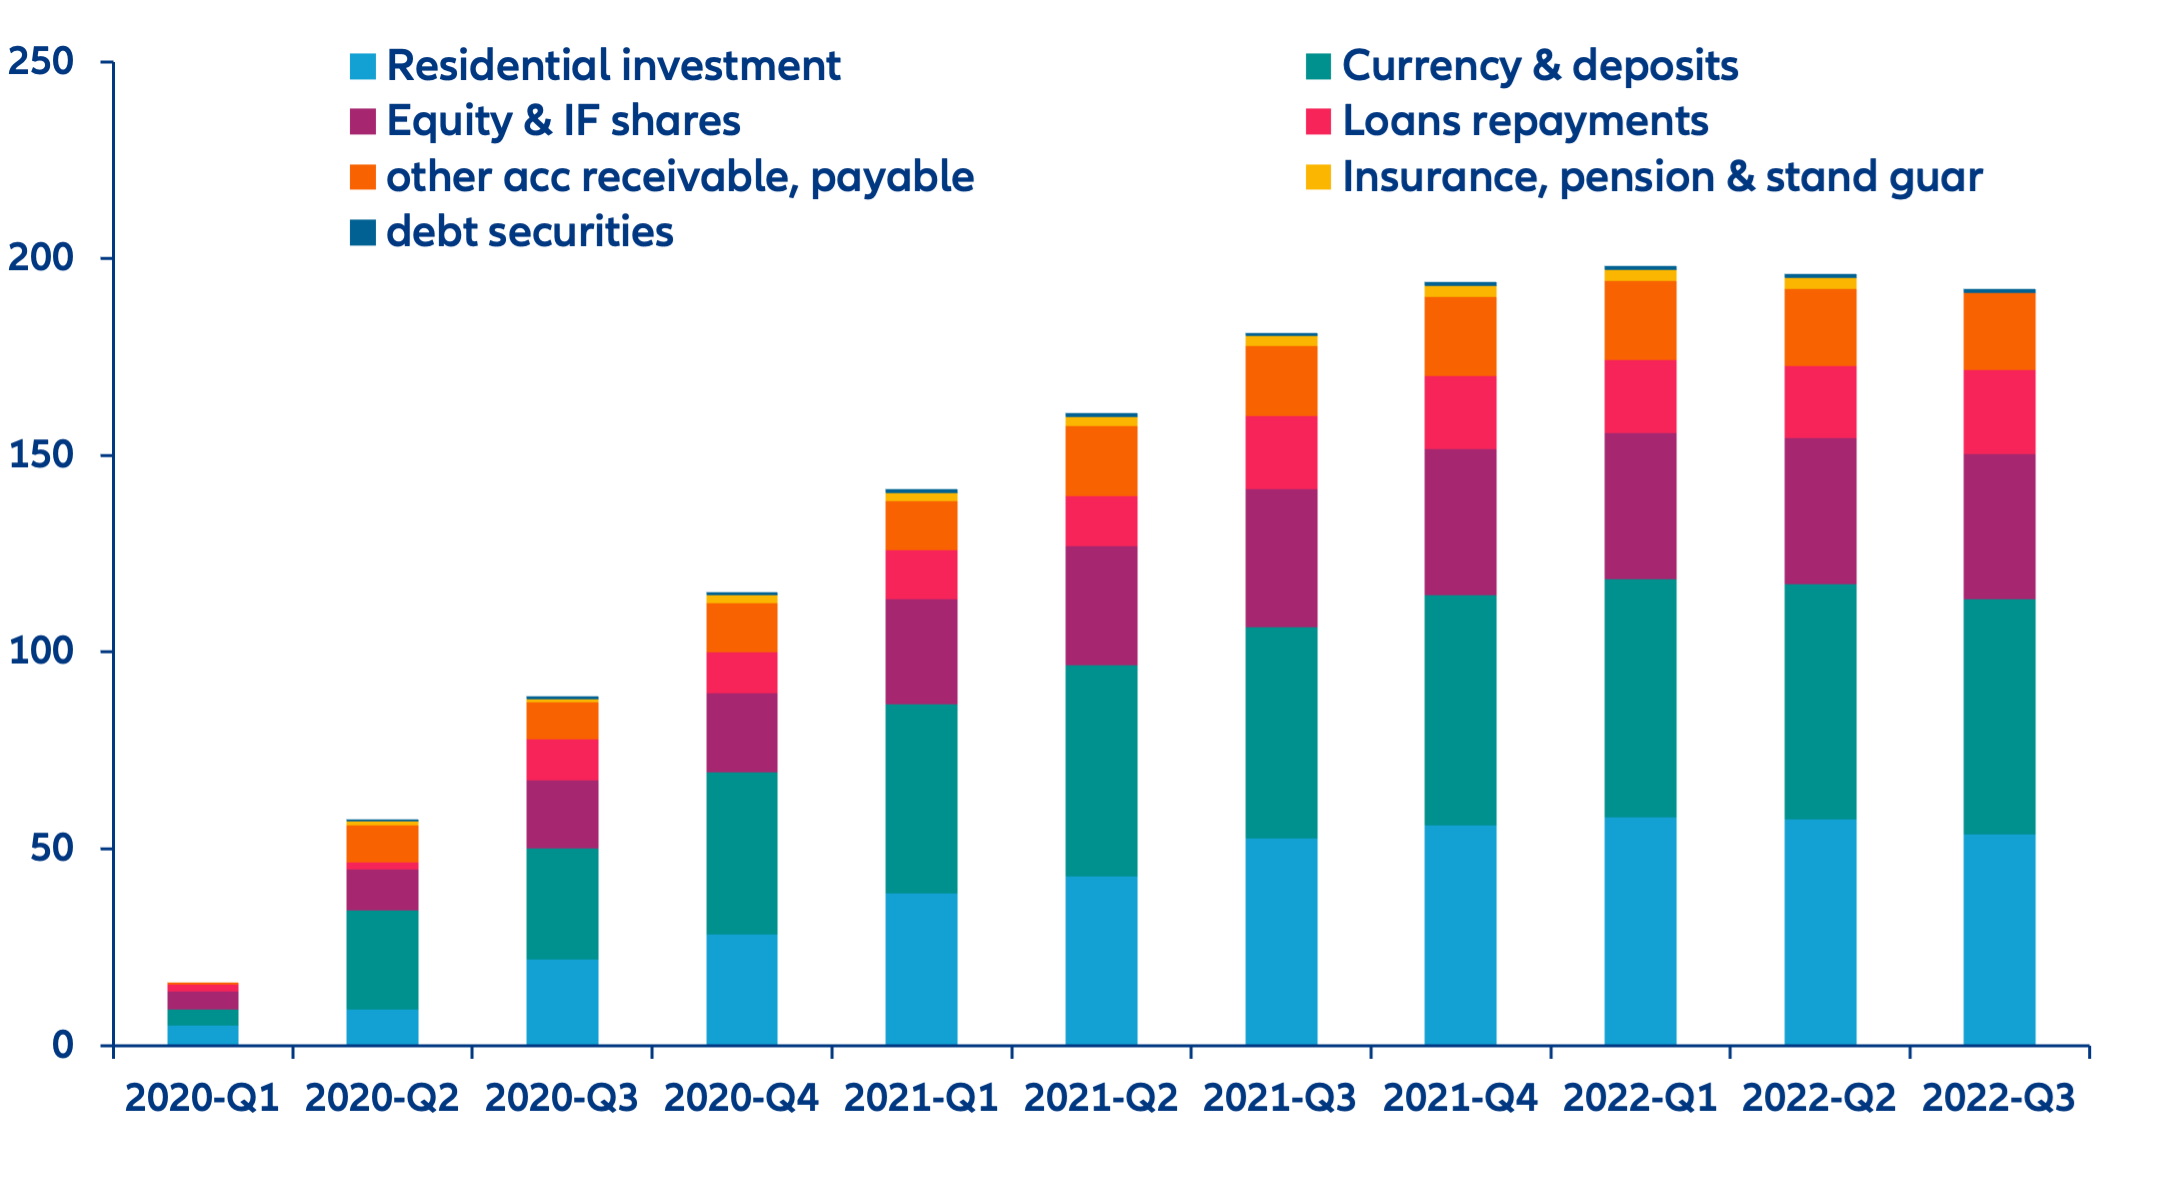
\includegraphics[width=.8\textwidth]{Core/1.Savings/img/xSpainAL.png}
    \label{figure:SpainAL}
\end{figure}
%\vspace{-0.5cm}
Furthermore, the data shows that only Spain and the US show some negative quarters of net investment in loans repayments. Thus, according to our methodology, only these two countries show overall tendency of households to actively direct these excess savings towards repaying their debt. It Spain net loans repayments happened in Q1 and Q3 of both 2020 and 2021 but also in Q3 2022, while in the US it was in the first semester of 2020 and in Q1 2021. Our computation suggest that between 2020 and late 2022, 15\% of excess savings have been invested towards loan repayments in Spain and only 2\% in the US.

In hindsight, the methodology still lacks efficiency and is probably too rough in several aspects (for instance negative saving flows are hard to account for). It does not appear to best the best decision to consider that when saving flows are negative households dig in their savings to fund investments, but rather direct these funds towards consumption. 
However, it was really interesting to work on this topic and to propose a methodology of our own. As there was a lot of national accounts topics that I had to learn about and finding the data sometimes being a challenge in itself, I still wanted to include these results with room for improvement.

\newpage

\subsection{Summary of key findings}
\begin{itemize}
    \item The stock of household excess savings is still large in European countries and the US in absolute terms. This huge stock of savings has barely started to come down in European countries while American households have started depleting savings as early as Q4 2021. 
    \item Excess savings are unevenly distributed across income groups, with the bottom 40\% of the spectrum having little to no excess savings left as of early 2023 and in the current economic situation higher income households are less likely to spend their excess savings which they consider more as assets rather than extra income to be spent.
    \item US consumption spending has outpaced European’s in the aftermath of the pandemic but this means that the US stock of excess savings is now depleting fast. Increasing strains on US households’ finances mean that excess savings are to remain under heavy pressure and potentially fully deplete throughout the year.
\end{itemize}